\newcommand{\fwb}{2.45cm}
\newcommand{\fwh}{2cm}
\begin{figure}
\centering
\begin{tabular}{c|c|c}
\rotatebox{90}{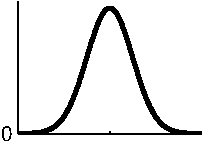
\includegraphics[width=\fwh,height=\fwb]{../figures/structure_examples/se_kernel}} &  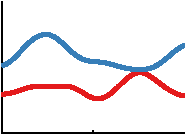
\includegraphics[width=\fwb,height=\fwh]{../figures/structure_examples/se_kernel_draws} & 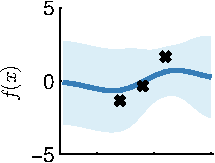
\includegraphics[width=\fwb,height=\fwh]{../figures/structure_examples/se_kernel_post} \\
\rotatebox{90}{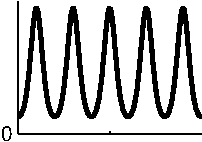
\includegraphics[width=\fwh,height=\fwb]{../figures/structure_examples/per_kernel}} &  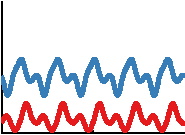
\includegraphics[width=\fwb,height=\fwh]{../figures/structure_examples/per_kernel_draws} & 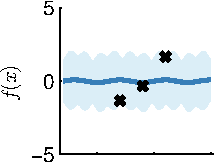
\includegraphics[width=\fwb,height=\fwh]{../figures/structure_examples/per_kernel_post} \\
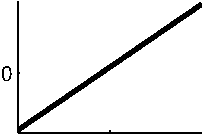
\includegraphics[width=\fwb,height=\fwh]{../figures/structure_examples/lin_kernel} &  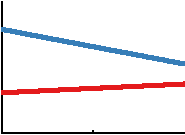
\includegraphics[width=\fwb,height=\fwh]{../figures/structure_examples/lin_kernel_draws} & 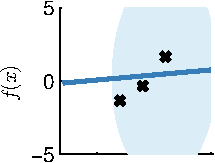
\includegraphics[width=\fwb,height=\fwh]{../figures/structure_examples/lin_kernel_post} \\
\rotatebox{90}{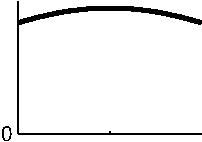
\includegraphics[width=\fwh,height=\fwb]{../figures/structure_examples/longse_kernel}} &  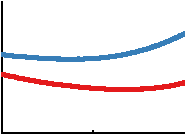
\includegraphics[width=\fwb,height=\fwh]{../figures/structure_examples/longse_kernel_draws} & 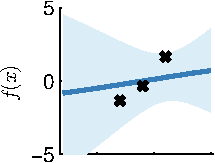
\includegraphics[width=\fwb,height=\fwh]{../figures/structure_examples/longse_kernel_post} \\
base kernel & draws from GP & GP posterior
\end{tabular}
\caption{ Properties of basic kernels.}
\label{fig:basic_kernels}
\end{figure}
